Le phénomène {\it d'adsorption} décrit le piégeage des molécules (de masse $m$) d'un gaz (à trois dimensions) sur la surface d'un solide (à deux dimensions) appelé substrat.  \`A l'équilibre thermodynamique, les molécules du gaz passent réversiblement de la phase gazeuse à la phase adsorbée.  Le nombre de molécules de la phase adsorbée n'étant pas constant, il est naturel d'utiliser le formalisme grand-canonique pour décrire cette phase 2D, dont le potentiel chimique est fixé par le gaz qui joue ici le rôle d'un grand réservoir. Soient $\rho$ la densité particulaire du gaz et $T$ sa température. On admet que le gaz est suffisamment dilué pour se comporter comme un gaz parfait. On note $h$ la constante de Planck.

\question
Rappeler l'expression du potentiel chimique $\mu$ du gaz en fonction de $\rho, k_B T$ et de la longueur d'onde thermique de de Broglie $\Lambda=\frac{h}{\sqrt{2\pi m k_B T}}$. En déduire que $\exp(\beta \mu)=\frac{P}{P_0(T)}$ où $P$ est la pression du gaz et $P_0(T)$ une fonction de la température seulement que l'on explicitera.

Dans le modèle de Langmuir les molécules adsorbées peuvent se fixer sur des sites réactionnels du substrat par une liaison chimique d'énergie $-\epsilon_0$.  Les $M$ sites du substrat sont discernables, indépendants et identiques et ne peuvent accueillir chacun au plus qu'une molécule.  On notera $n_i$ le nombre d'occupation du site $i$.  Le potentiel chimique des molécules de la phase adsorbée est égal $\mu$.

\question
Donner l'expression du nombre $N_a$ de molécules adsorbées et l'expression de l'énergie $E_a$ de la phase adsorbée en fonction des $\{n_i\}_{1\leq i \leq M}$ et de $\epsilon_0$.

\question
Calculer la grande fonction de partition $\Xi (T,M,\mu)$ de la phase adsorbée dans l'ensemble grand-canonique. On montrera qu'elle s'exprime comme $\Xi=\xi(T,\mu)^M$ où $\xi=1+e^{\beta(\mu+\epsilon_0)}$ est la grande fonction de partition d'un seul site.

\question
En déduire le nombre moyen $\langle N_a \rangle$ de molécules adsorbées ainsi que le taux de couverture de la surface $\theta=\frac{\langle N_a \rangle}{M}$  en fonction de $T$ et $\mu$. Montrer ensuite que
\begin{equation} \label{lang} 
  \displaystyle \theta(P,T)=   \displaystyle{\frac{P} {P+ P_0(T) {\rm e}^{-\beta \epsilon_0}}}
\end{equation}
Tracer l'allure de $\theta$ en fonction de la pression à température
fixée (courbe appelée isotherme de Langmuir).

\question
Les résultats d'une étude sur l'adsorption du trifluorométhane dans un zéolithe, sont présentés sur la figure \ref{FigLangmuir}. \'Evaluer $\epsilon_0$, l'énergie de liaison entre une molécule et le substrat.

\begin{center}
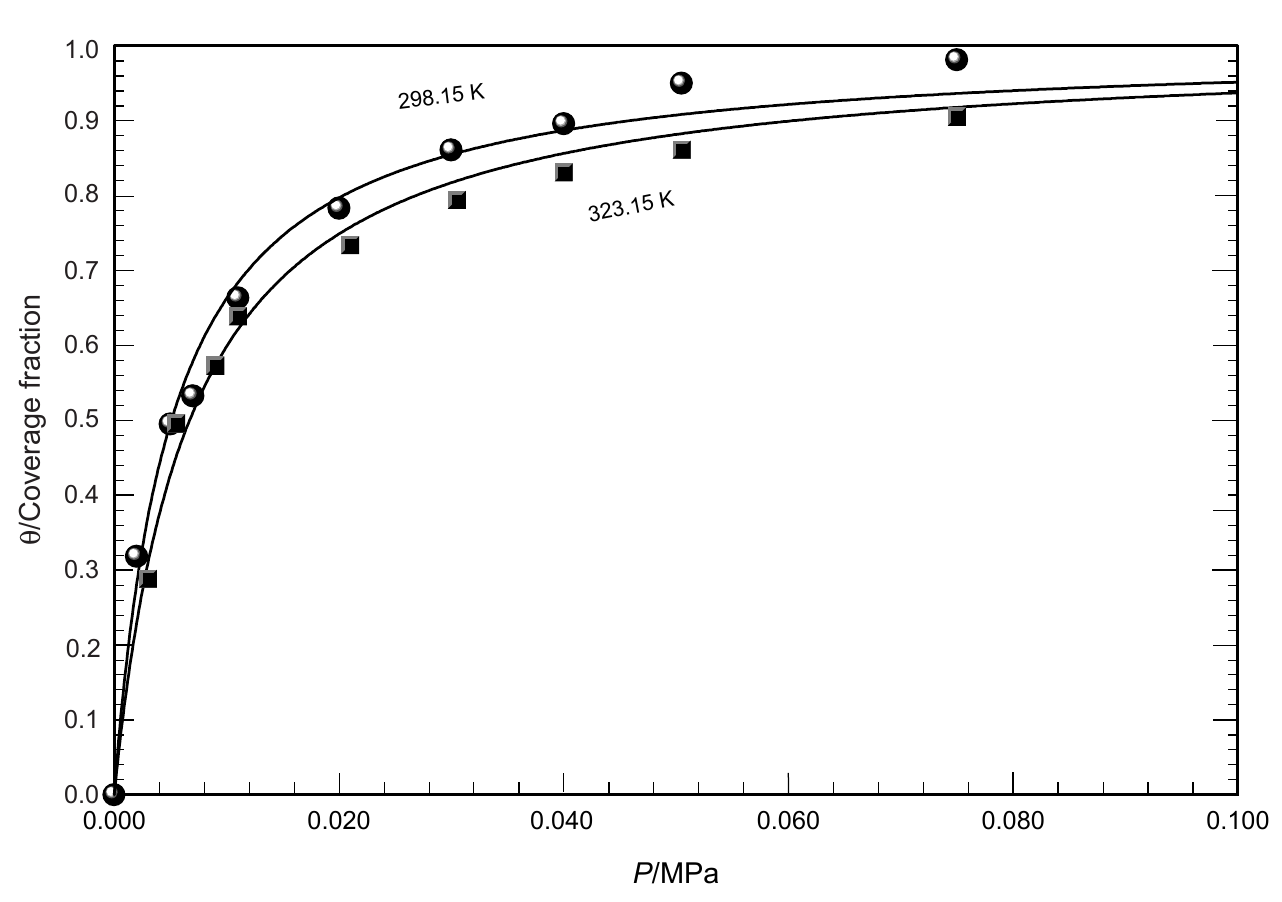
\includegraphics{../Fig/Langmuir} \\
\textit{Taux d'adsorption $\theta(P)$  de CHF$_3$ en fonction de la pression $P$ (en MPa) à $T=298$ K et $T=323$ K dans une zéolithe. Les courbes représentent des isothermes de Langmuir données par l'équation (\ref{lang}) avec $P_0 \simeq 1,8$ bar (d'après M.B. Shiflett et al., Adsorption Science and Technology {\bf 31}, 59 (2013)). \label{FigLangmuir}}
\end{center}
